\chapter{Experimental setup for SAXS measurements}
\label{chap:experimental_setup}

\section{BESSY II}

\section{FCM Beamline}
\subsection{Transmission measurements}
calibrated diodes, SYRES II????

\section{Small-angle X-ray scattering}
The measurements were performed at the four-crystal monochromator beamline in the PTB laboratory at the electron storage ring BESSY II (Berlin, \emph{Germany}), which provides highly intense, collimated synchrotron radiation focused on the sample and collimated into a \(0.5\) mm circular spot by Ge pinholes situated between the sample and the monochromator with an energy resolving
power \( E/\Delta E \) of \( 10^4 \). To measure the total flux and sample transmission, photodiodes were used which were calibrated against a cryogenic electric substitution radiometer with a relative uncertainty of \( 1\,\% \) \cite{Krumrey2001}.

The rectangular capillary is placed in a sample holder which allows the movement with micrometer precision in the directions perpendicular to the incoming beam, as depicted in figure \ref{fig:0}. In order to determine the central vertical capillary axis, a horizontal X-ray transmission scan is performed at two different vertical positions of the capillary spaced by 20 mm. The central vertical axis can be drawn from the centers of both measurements and the sample can be moved along this axis by the simultaneous operation of the vertical and horizontal motors.

The sample was moved in steps of 0.5 mm along the central vertical capillary axis and exposed at each position for 45 seconds. At these positions, the solution transmittances were previously measured and the suspending medium electron density calibrated. The measured scattering curve is an average over a range of solvent electron densities associated with the beam size. The momentum transfer \(q\) of the scattering curves was calculated using
\begin{equation}
q=\frac{4\pi E}{hc}\sin\theta ,
\end{equation}
where \(\theta\) is half of the scattering angle, \(h\) is the Planck constant and \(c\) is the speed of light. The incident photon energy \(E = \left(8800.0  \pm 0.8\right)\) eV was chosen to be higher than the photon energy for the transmission measurements to improve the recorded statistics, due to a ca. \(150\) higher transmission \cite{Henke1993}. The scattered X-ray photons were collected with a vacuum-compatible Pilatus 1M hybrid-pixel detector (Dectris Ltd, (Baden, \emph{Switzerland})) with a pixel size of \(d = \left(172.1  \pm 0.2\right) \; \mu \)m at a distance \(L = \left(4540.2  \pm 0.8\right)\) mm from the capillaries, determined by triangulation using a calibrated length measurement system \cite{Wernecke2014}. The obtained scattering curve was normalized to the exposure time and the incident intensity, measured by means of a calibrated transparent silicon diode.  In total, 40 scattering curves with different solvent electron densities were measured at two different times \(t_1=\)78 min and \(t_2=\)156 min after filling the capillaries.
\subsection{Pilatus detector}
high dynamic range
noise free
\subsection{HZB SAXS setup}
\subsubsection{distance calibration}
10-4 uncertainty

\subsection{Radial integration and error propagation}
\subsection{Absolute intensity calibration}
\subsubsection{Flux monitor}
thin diode
\subsubsection{Detector efficiceny}
pilatus and thin diode

\section{Continuous contrast variation}
\subsection{Filling of capilaries}
galden at bottom, reference layer
\subsubsection{Capillary homogeneity}
Hilgenberg

\subsection{Calibration of solvent density and finding of main axis}
The transmitted intensity through the sample is recorded at a photon energy of \(E = (5500.0 \pm  0.5)\) eV for 10 seconds at each position. The measurement consists of 20 points spaced 0.5 mm along the central vertical axis of the capillary. The overall X-ray transmission measurement requires approximately 5 minutes, which is within the calculated diffusion timescale of the aqueous sucrose solution. The solvent electron density profile within the density gradient capillary derived from this measurement is depicted in figure \ref{fig:1}. A uniform thickness of the capillary within $0.5\,\%$ along this axis was determined by measuring the X-ray transmission of an empty capillary. The associated uncertainty in the sample transmission measurement is below $4\,\%$. The sample thickness is assumed to be constant. This transmission measurement is performed both immediately before and after recording the scattering patterns, which takes 15 minutes to complete. The transmittance values used for the density calibration are then linearly interpolated between both data sets taking into account the time-dependence. These values can be converted to solvent electron densities via the Beer-Lambert law, which relates the density of the solution with the transmitted intensity:
\begin{equation}
  \rho(z) = A \left( \ln{I_0} - \ln{I(z)} \right) .
\end{equation}
Here \(\rho\) is the electron density of the suspending medium, $I$ and $I_0$ are the transmitted and incoming intensities respectively and $A$ is a factor determined by the reference values of the solvent electron density at the vertical limits of the capillary at the initial time. The sucrose concentration in solution expressed as the mass fraction \( M \) at these reference points can be converted to electron densities with the empirical formula \( \rho=1.2681M+333.19 \) nm\(^{-3}\) \cite{Haynes2012}. The suspending medium electron density shows a maximum uncertainty of 1 nm$^{-3}$ associated with the vertical size of the focused X-ray beam.

\begin{figure}%[htbp]
	\centering
		\subfloat[Isoscattering point positions]{\resizebox{0.45\linewidth}{!}{% GNUPLOT: LaTeX picture with Postscript
\begingroup
  \makeatletter
  \providecommand\color[2][]{%
    \GenericError{(gnuplot) \space\space\space\@spaces}{%
      Package color not loaded in conjunction with
      terminal option `colourtext'%
    }{See the gnuplot documentation for explanation.%
    }{Either use 'blacktext' in gnuplot or load the package
      color.sty in LaTeX.}%
    \renewcommand\color[2][]{}%
  }%
  \providecommand\includegraphics[2][]{%
    \GenericError{(gnuplot) \space\space\space\@spaces}{%
      Package graphicx or graphics not loaded%
    }{See the gnuplot documentation for explanation.%
    }{The gnuplot epslatex terminal needs graphicx.sty or graphics.sty.}%
    \renewcommand\includegraphics[2][]{}%
  }%
  \providecommand\rotatebox[2]{#2}%
  \@ifundefined{ifGPcolor}{%
    \newif\ifGPcolor
    \GPcolortrue
  }{}%
  \@ifundefined{ifGPblacktext}{%
    \newif\ifGPblacktext
    \GPblacktextfalse
  }{}%
  % define a \g@addto@macro without @ in the name:
  \let\gplgaddtomacro\g@addto@macro
  % define empty templates for all commands taking text:
  \gdef\gplbacktext{}%
  \gdef\gplfronttext{}%
  \makeatother
  \ifGPblacktext
    % no textcolor at all
    \def\colorrgb#1{}%
    \def\colorgray#1{}%
  \else
    % gray or color?
    \ifGPcolor
      \def\colorrgb#1{\color[rgb]{#1}}%
      \def\colorgray#1{\color[gray]{#1}}%
      \expandafter\def\csname LTw\endcsname{\color{white}}%
      \expandafter\def\csname LTb\endcsname{\color{black}}%
      \expandafter\def\csname LTa\endcsname{\color{black}}%
      \expandafter\def\csname LT0\endcsname{\color[rgb]{1,0,0}}%
      \expandafter\def\csname LT1\endcsname{\color[rgb]{0,1,0}}%
      \expandafter\def\csname LT2\endcsname{\color[rgb]{0,0,1}}%
      \expandafter\def\csname LT3\endcsname{\color[rgb]{1,0,1}}%
      \expandafter\def\csname LT4\endcsname{\color[rgb]{0,1,1}}%
      \expandafter\def\csname LT5\endcsname{\color[rgb]{1,1,0}}%
      \expandafter\def\csname LT6\endcsname{\color[rgb]{0,0,0}}%
      \expandafter\def\csname LT7\endcsname{\color[rgb]{1,0.3,0}}%
      \expandafter\def\csname LT8\endcsname{\color[rgb]{0.5,0.5,0.5}}%
    \else
      % gray
      \def\colorrgb#1{\color{black}}%
      \def\colorgray#1{\color[gray]{#1}}%
      \expandafter\def\csname LTw\endcsname{\color{white}}%
      \expandafter\def\csname LTb\endcsname{\color{black}}%
      \expandafter\def\csname LTa\endcsname{\color{black}}%
      \expandafter\def\csname LT0\endcsname{\color{black}}%
      \expandafter\def\csname LT1\endcsname{\color{black}}%
      \expandafter\def\csname LT2\endcsname{\color{black}}%
      \expandafter\def\csname LT3\endcsname{\color{black}}%
      \expandafter\def\csname LT4\endcsname{\color{black}}%
      \expandafter\def\csname LT5\endcsname{\color{black}}%
      \expandafter\def\csname LT6\endcsname{\color{black}}%
      \expandafter\def\csname LT7\endcsname{\color{black}}%
      \expandafter\def\csname LT8\endcsname{\color{black}}%
    \fi
  \fi
    \setlength{\unitlength}{0.0500bp}%
    \ifx\gptboxheight\undefined%
      \newlength{\gptboxheight}%
      \newlength{\gptboxwidth}%
      \newsavebox{\gptboxtext}%
    \fi%
    \setlength{\fboxrule}{0.5pt}%
    \setlength{\fboxsep}{1pt}%
\begin{picture}(8502.00,4534.00)%
    \gplgaddtomacro\gplbacktext{%
      \csname LTb\endcsname%
      \put(550,815){\makebox(0,0)[r]{\strut{}$0$}}%
      \csname LTb\endcsname%
      \put(550,1239){\makebox(0,0)[r]{\strut{}$5$}}%
      \csname LTb\endcsname%
      \put(550,1663){\makebox(0,0)[r]{\strut{}$10$}}%
      \csname LTb\endcsname%
      \put(550,2087){\makebox(0,0)[r]{\strut{}$15$}}%
      \csname LTb\endcsname%
      \put(550,2511){\makebox(0,0)[r]{\strut{}$20$}}%
      \csname LTb\endcsname%
      \put(550,2935){\makebox(0,0)[r]{\strut{}$25$}}%
      \csname LTb\endcsname%
      \put(550,3359){\makebox(0,0)[r]{\strut{}$30$}}%
      \csname LTb\endcsname%
      \put(550,3783){\makebox(0,0)[r]{\strut{}$35$}}%
      \csname LTb\endcsname%
      \put(550,4206){\makebox(0,0)[r]{\strut{}$40$}}%
      \csname LTb\endcsname%
      \put(682,484){\makebox(0,0){\strut{}$0$}}%
      \csname LTb\endcsname%
      \put(1456,484){\makebox(0,0){\strut{}$2$}}%
      \csname LTb\endcsname%
      \put(2230,484){\makebox(0,0){\strut{}$4$}}%
      \csname LTb\endcsname%
      \put(3004,484){\makebox(0,0){\strut{}$6$}}%
      \csname LTb\endcsname%
      \put(3778,484){\makebox(0,0){\strut{}$8$}}%
      \csname LTb\endcsname%
      \put(4552,484){\makebox(0,0){\strut{}$10$}}%
      \csname LTb\endcsname%
      \put(5326,484){\makebox(0,0){\strut{}$12$}}%
      \csname LTb\endcsname%
      \put(6100,484){\makebox(0,0){\strut{}$14$}}%
      \put(6425,4187){\makebox(0,0)[l]{\strut{}$1.2$}}%
      \put(6425,3202){\makebox(0,0)[l]{\strut{}$2$}}%
      \put(6425,1864){\makebox(0,0)[l]{\strut{}$4$}}%
      \put(6425,785){\makebox(0,0)[l]{\strut{}$7$}}%
    }%
    \gplgaddtomacro\gplfronttext{%
      \csname LTb\endcsname%
      \put(176,2486){\rotatebox{-270}{\makebox(0,0){\strut{}Particle Mass Concentration / $\%$}}}%
      \put(6732,2486){\rotatebox{270}{\makebox(0,0){\strut{}X-ray Transmission / $\%$}}}%
      \put(3487,154){\makebox(0,0){\strut{}Vertical Position / mm}}%
      \csname LTb\endcsname%
      \put(7505,704){\makebox(0,0)[l]{\strut{}\smaller 100}}%
      \put(7505,1213){\makebox(0,0)[l]{\strut{}\smaller 120}}%
      \put(7505,1722){\makebox(0,0)[l]{\strut{}\smaller 140}}%
      \put(7505,2231){\makebox(0,0)[l]{\strut{}\smaller 160}}%
      \put(7505,2741){\makebox(0,0)[l]{\strut{}\smaller 180}}%
      \put(7505,3250){\makebox(0,0)[l]{\strut{}\smaller 200}}%
      \put(7505,3759){\makebox(0,0)[l]{\strut{}\smaller 220}}%
      \put(7505,4269){\makebox(0,0)[l]{\strut{}\smaller 240}}%
      \put(7968,2486){\rotatebox{270}{\makebox(0,0){\strut{}\smaller Diffusion Time / min}}}%
    }%
    \gplbacktext
    \put(0,0){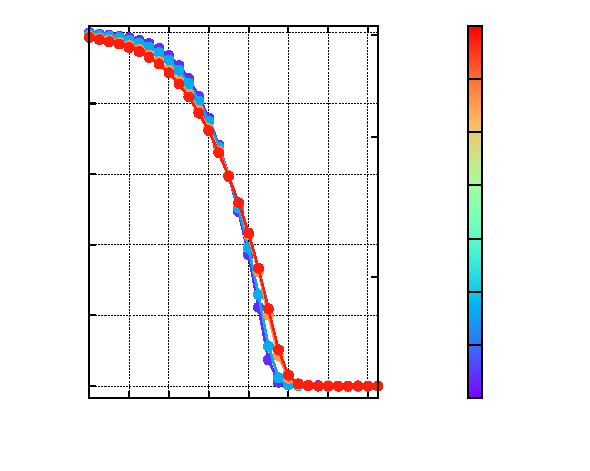
\includegraphics{LudoxHS40TransmissionCalibration}}%
    \gplfronttext
  \end{picture}%
\endgroup
}\label{fig:LudoxHS40TransmissionCalibration}}
		\subfloat[Scattering curves]{\resizebox{0.45\linewidth}{!}{% GNUPLOT: LaTeX picture with Postscript
\begingroup
  \makeatletter
  \providecommand\color[2][]{%
    \GenericError{(gnuplot) \space\space\space\@spaces}{%
      Package color not loaded in conjunction with
      terminal option `colourtext'%
    }{See the gnuplot documentation for explanation.%
    }{Either use 'blacktext' in gnuplot or load the package
      color.sty in LaTeX.}%
    \renewcommand\color[2][]{}%
  }%
  \providecommand\includegraphics[2][]{%
    \GenericError{(gnuplot) \space\space\space\@spaces}{%
      Package graphicx or graphics not loaded%
    }{See the gnuplot documentation for explanation.%
    }{The gnuplot epslatex terminal needs graphicx.sty or graphics.sty.}%
    \renewcommand\includegraphics[2][]{}%
  }%
  \providecommand\rotatebox[2]{#2}%
  \@ifundefined{ifGPcolor}{%
    \newif\ifGPcolor
    \GPcolortrue
  }{}%
  \@ifundefined{ifGPblacktext}{%
    \newif\ifGPblacktext
    \GPblacktextfalse
  }{}%
  % define a \g@addto@macro without @ in the name:
  \let\gplgaddtomacro\g@addto@macro
  % define empty templates for all commands taking text:
  \gdef\gplbacktext{}%
  \gdef\gplfronttext{}%
  \makeatother
  \ifGPblacktext
    % no textcolor at all
    \def\colorrgb#1{}%
    \def\colorgray#1{}%
  \else
    % gray or color?
    \ifGPcolor
      \def\colorrgb#1{\color[rgb]{#1}}%
      \def\colorgray#1{\color[gray]{#1}}%
      \expandafter\def\csname LTw\endcsname{\color{white}}%
      \expandafter\def\csname LTb\endcsname{\color{black}}%
      \expandafter\def\csname LTa\endcsname{\color{black}}%
      \expandafter\def\csname LT0\endcsname{\color[rgb]{1,0,0}}%
      \expandafter\def\csname LT1\endcsname{\color[rgb]{0,1,0}}%
      \expandafter\def\csname LT2\endcsname{\color[rgb]{0,0,1}}%
      \expandafter\def\csname LT3\endcsname{\color[rgb]{1,0,1}}%
      \expandafter\def\csname LT4\endcsname{\color[rgb]{0,1,1}}%
      \expandafter\def\csname LT5\endcsname{\color[rgb]{1,1,0}}%
      \expandafter\def\csname LT6\endcsname{\color[rgb]{0,0,0}}%
      \expandafter\def\csname LT7\endcsname{\color[rgb]{1,0.3,0}}%
      \expandafter\def\csname LT8\endcsname{\color[rgb]{0.5,0.5,0.5}}%
    \else
      % gray
      \def\colorrgb#1{\color{black}}%
      \def\colorgray#1{\color[gray]{#1}}%
      \expandafter\def\csname LTw\endcsname{\color{white}}%
      \expandafter\def\csname LTb\endcsname{\color{black}}%
      \expandafter\def\csname LTa\endcsname{\color{black}}%
      \expandafter\def\csname LT0\endcsname{\color{black}}%
      \expandafter\def\csname LT1\endcsname{\color{black}}%
      \expandafter\def\csname LT2\endcsname{\color{black}}%
      \expandafter\def\csname LT3\endcsname{\color{black}}%
      \expandafter\def\csname LT4\endcsname{\color{black}}%
      \expandafter\def\csname LT5\endcsname{\color{black}}%
      \expandafter\def\csname LT6\endcsname{\color{black}}%
      \expandafter\def\csname LT7\endcsname{\color{black}}%
      \expandafter\def\csname LT8\endcsname{\color{black}}%
    \fi
  \fi
    \setlength{\unitlength}{0.0500bp}%
    \ifx\gptboxheight\undefined%
      \newlength{\gptboxheight}%
      \newlength{\gptboxwidth}%
      \newsavebox{\gptboxtext}%
    \fi%
    \setlength{\fboxrule}{0.5pt}%
    \setlength{\fboxsep}{1pt}%
\begin{picture}(8502.00,4534.00)%
    \gplgaddtomacro\gplbacktext{%
      \csname LTb\endcsname%
      \put(594,1050){\makebox(0,0)[r]{\strut{}$335$}}%
      \csname LTb\endcsname%
      \put(594,1614){\makebox(0,0)[r]{\strut{}$340$}}%
      \csname LTb\endcsname%
      \put(594,2178){\makebox(0,0)[r]{\strut{}$345$}}%
      \csname LTb\endcsname%
      \put(594,2742){\makebox(0,0)[r]{\strut{}$350$}}%
      \csname LTb\endcsname%
      \put(594,3306){\makebox(0,0)[r]{\strut{}$355$}}%
      \csname LTb\endcsname%
      \put(594,3870){\makebox(0,0)[r]{\strut{}$360$}}%
      \csname LTb\endcsname%
      \put(951,484){\makebox(0,0){\strut{}$0$}}%
      \csname LTb\endcsname%
      \put(1851,484){\makebox(0,0){\strut{}$2$}}%
      \csname LTb\endcsname%
      \put(2751,484){\makebox(0,0){\strut{}$4$}}%
      \csname LTb\endcsname%
      \put(3651,484){\makebox(0,0){\strut{}$6$}}%
      \csname LTb\endcsname%
      \put(4551,484){\makebox(0,0){\strut{}$8$}}%
      \csname LTb\endcsname%
      \put(5451,484){\makebox(0,0){\strut{}$10$}}%
      \put(6033,3996){\makebox(0,0)[l]{\strut{}$0.027$}}%
      \put(6033,3109){\makebox(0,0)[l]{\strut{}$0.028$}}%
      \put(6033,1835){\makebox(0,0)[l]{\strut{}$0.0295$}}%
      \put(6033,1022){\makebox(0,0)[l]{\strut{}$0.0305$}}%
    }%
    \gplgaddtomacro\gplfronttext{%
      \csname LTb\endcsname%
      \put(220,2486){\rotatebox{-270}{\makebox(0,0){\strut{}Solvent electron density / nm$^{-3}$}}}%
      \put(6736,2486){\rotatebox{270}{\makebox(0,0){\strut{}X-ray Transmission / $\%$}}}%
      \put(3313,154){\makebox(0,0){\strut{}Vertical Position / mm}}%
      \csname LTb\endcsname%
      \put(7476,704){\makebox(0,0)[l]{\strut{}\smaller 100}}%
      \put(7476,1213){\makebox(0,0)[l]{\strut{}\smaller 120}}%
      \put(7476,1722){\makebox(0,0)[l]{\strut{}\smaller 140}}%
      \put(7476,2231){\makebox(0,0)[l]{\strut{}\smaller 160}}%
      \put(7476,2741){\makebox(0,0)[l]{\strut{}\smaller 180}}%
      \put(7476,3250){\makebox(0,0)[l]{\strut{}\smaller 200}}%
      \put(7476,3759){\makebox(0,0)[l]{\strut{}\smaller 220}}%
      \put(7476,4269){\makebox(0,0)[l]{\strut{}\smaller 240}}%
      \put(7939,2486){\rotatebox{270}{\makebox(0,0){\strut{}\smaller Diffusion Time / min}}}%
    }%
    \gplbacktext
    \put(0,0){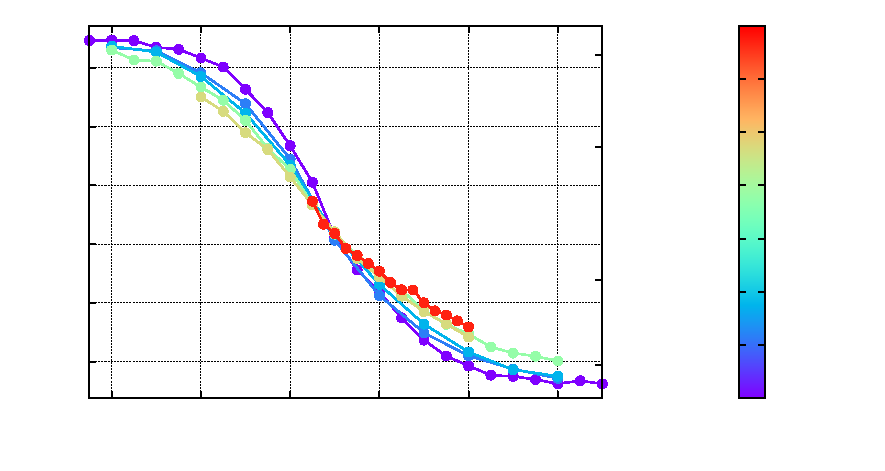
\includegraphics{KiskerTransmissionCalibration}}%
    \gplfronttext
  \end{picture}%
\endgroup
}\label{fig:KiskerTransmissionCalibration}}
	\caption{Typical measurement of particles with different diffusion timescale: Sucrose (with Kisker NPs) measured at 5500 eV and Colloids (Ludox HS40) mesaured at 8000eV}
\end{figure}

\begin{figure}%[htbp]
	\centering
		\subfloat[Transmission calculation]{\resizebox{0.44\linewidth}{!}{% GNUPLOT: LaTeX picture with Postscript
\begingroup
  \makeatletter
  \providecommand\color[2][]{%
    \GenericError{(gnuplot) \space\space\space\@spaces}{%
      Package color not loaded in conjunction with
      terminal option `colourtext'%
    }{See the gnuplot documentation for explanation.%
    }{Either use 'blacktext' in gnuplot or load the package
      color.sty in LaTeX.}%
    \renewcommand\color[2][]{}%
  }%
  \providecommand\includegraphics[2][]{%
    \GenericError{(gnuplot) \space\space\space\@spaces}{%
      Package graphicx or graphics not loaded%
    }{See the gnuplot documentation for explanation.%
    }{The gnuplot epslatex terminal needs graphicx.sty or graphics.sty.}%
    \renewcommand\includegraphics[2][]{}%
  }%
  \providecommand\rotatebox[2]{#2}%
  \@ifundefined{ifGPcolor}{%
    \newif\ifGPcolor
    \GPcolortrue
  }{}%
  \@ifundefined{ifGPblacktext}{%
    \newif\ifGPblacktext
    \GPblacktextfalse
  }{}%
  % define a \g@addto@macro without @ in the name:
  \let\gplgaddtomacro\g@addto@macro
  % define empty templates for all commands taking text:
  \gdef\gplbacktext{}%
  \gdef\gplfronttext{}%
  \makeatother
  \ifGPblacktext
    % no textcolor at all
    \def\colorrgb#1{}%
    \def\colorgray#1{}%
  \else
    % gray or color?
    \ifGPcolor
      \def\colorrgb#1{\color[rgb]{#1}}%
      \def\colorgray#1{\color[gray]{#1}}%
      \expandafter\def\csname LTw\endcsname{\color{white}}%
      \expandafter\def\csname LTb\endcsname{\color{black}}%
      \expandafter\def\csname LTa\endcsname{\color{black}}%
      \expandafter\def\csname LT0\endcsname{\color[rgb]{1,0,0}}%
      \expandafter\def\csname LT1\endcsname{\color[rgb]{0,1,0}}%
      \expandafter\def\csname LT2\endcsname{\color[rgb]{0,0,1}}%
      \expandafter\def\csname LT3\endcsname{\color[rgb]{1,0,1}}%
      \expandafter\def\csname LT4\endcsname{\color[rgb]{0,1,1}}%
      \expandafter\def\csname LT5\endcsname{\color[rgb]{1,1,0}}%
      \expandafter\def\csname LT6\endcsname{\color[rgb]{0,0,0}}%
      \expandafter\def\csname LT7\endcsname{\color[rgb]{1,0.3,0}}%
      \expandafter\def\csname LT8\endcsname{\color[rgb]{0.5,0.5,0.5}}%
    \else
      % gray
      \def\colorrgb#1{\color{black}}%
      \def\colorgray#1{\color[gray]{#1}}%
      \expandafter\def\csname LTw\endcsname{\color{white}}%
      \expandafter\def\csname LTb\endcsname{\color{black}}%
      \expandafter\def\csname LTa\endcsname{\color{black}}%
      \expandafter\def\csname LT0\endcsname{\color{black}}%
      \expandafter\def\csname LT1\endcsname{\color{black}}%
      \expandafter\def\csname LT2\endcsname{\color{black}}%
      \expandafter\def\csname LT3\endcsname{\color{black}}%
      \expandafter\def\csname LT4\endcsname{\color{black}}%
      \expandafter\def\csname LT5\endcsname{\color{black}}%
      \expandafter\def\csname LT6\endcsname{\color{black}}%
      \expandafter\def\csname LT7\endcsname{\color{black}}%
      \expandafter\def\csname LT8\endcsname{\color{black}}%
    \fi
  \fi
  \setlength{\unitlength}{0.0500bp}%
  \begin{picture}(5668.00,4534.00)%
    \gplgaddtomacro\gplbacktext{%
      \csname LTb\endcsname%
      \put(946,939){\makebox(0,0)[r]{\strut{} 0.1}}%
      \csname LTb\endcsname%
      \put(946,2109){\makebox(0,0)[r]{\strut{} 1}}%
      \csname LTb\endcsname%
      \put(946,3280){\makebox(0,0)[r]{\strut{} 10}}%
      \csname LTb\endcsname%
      \put(1078,484){\makebox(0,0){\strut{} 5000}}%
      \csname LTb\endcsname%
      \put(1741,484){\makebox(0,0){\strut{} 6000}}%
      \csname LTb\endcsname%
      \put(2403,484){\makebox(0,0){\strut{} 7000}}%
      \csname LTb\endcsname%
      \put(3066,484){\makebox(0,0){\strut{} 8000}}%
      \csname LTb\endcsname%
      \put(3728,484){\makebox(0,0){\strut{} 9000}}%
      \csname LTb\endcsname%
      \put(4391,484){\makebox(0,0){\strut{} 10000}}%
      \colorrgb{0.00,0.00,1.00}%
      \put(4523,1224){\makebox(0,0)[l]{\strut{} 1.5}}%
      \colorrgb{0.00,0.00,1.00}%
      \put(4523,1967){\makebox(0,0)[l]{\strut{} 2}}%
      \colorrgb{0.00,0.00,1.00}%
      \put(4523,2709){\makebox(0,0)[l]{\strut{} 2.5}}%
      \colorrgb{0.00,0.00,1.00}%
      \put(4523,3452){\makebox(0,0)[l]{\strut{} 3}}%
      \colorrgb{0.00,0.00,1.00}%
      \put(4523,4195){\makebox(0,0)[l]{\strut{} 3.5}}%
      \csname LTb\endcsname%
      \put(176,2486){\rotatebox{-270}{\makebox(0,0){\strut{}X-ray Transmission / $\%$}}}%
      \colorrgb{0.00,0.00,1.00}%
      \put(5160,2486){\rotatebox{270}{\makebox(0,0){\strut{}Ratio}}}%
      \csname LTb\endcsname%
      \put(2734,154){\makebox(0,0){\strut{}Energy / eV}}%
    }%
    \gplgaddtomacro\gplfronttext{%
      \csname LTb\endcsname%
      \put(3800,2649){\makebox(0,0)[r]{\strut{}\smaller Capillary}}%
      \csname LTb\endcsname%
      \put(3800,2319){\makebox(0,0)[r]{\strut{}\smaller 0$\%$ sucrose}}%
      \csname LTb\endcsname%
      \put(3800,1989){\makebox(0,0)[r]{\strut{}\smaller 65$\%$ sucrose}}%
      \csname LTb\endcsname%
      \put(3800,1659){\makebox(0,0)[r]{\strut{}\smaller T$_{0\%}$/T$_{65\%}$}}%
    }%
    \gplbacktext
    \put(0,0){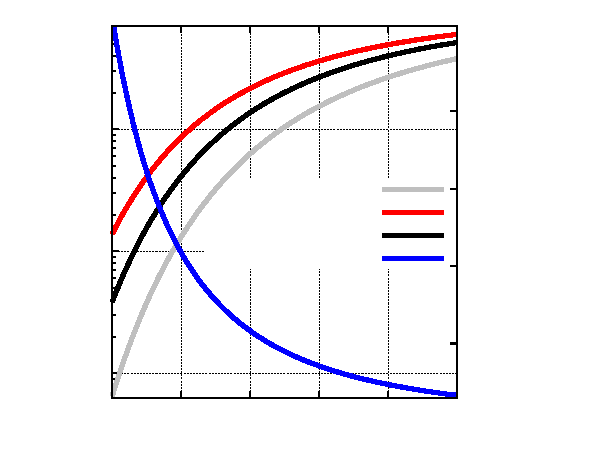
\includegraphics{EnergiesTransmissionCalibration}}%
    \gplfronttext
  \end{picture}%
\endgroup
}\label{fig:EnergiesTransmissionCalibration}}
		\subfloat[Calibrated sucrose concentration]{\resizebox{0.44\linewidth}{!}{% GNUPLOT: LaTeX picture with Postscript
\begingroup
  \makeatletter
  \providecommand\color[2][]{%
    \GenericError{(gnuplot) \space\space\space\@spaces}{%
      Package color not loaded in conjunction with
      terminal option `colourtext'%
    }{See the gnuplot documentation for explanation.%
    }{Either use 'blacktext' in gnuplot or load the package
      color.sty in LaTeX.}%
    \renewcommand\color[2][]{}%
  }%
  \providecommand\includegraphics[2][]{%
    \GenericError{(gnuplot) \space\space\space\@spaces}{%
      Package graphicx or graphics not loaded%
    }{See the gnuplot documentation for explanation.%
    }{The gnuplot epslatex terminal needs graphicx.sty or graphics.sty.}%
    \renewcommand\includegraphics[2][]{}%
  }%
  \providecommand\rotatebox[2]{#2}%
  \@ifundefined{ifGPcolor}{%
    \newif\ifGPcolor
    \GPcolortrue
  }{}%
  \@ifundefined{ifGPblacktext}{%
    \newif\ifGPblacktext
    \GPblacktextfalse
  }{}%
  % define a \g@addto@macro without @ in the name:
  \let\gplgaddtomacro\g@addto@macro
  % define empty templates for all commands taking text:
  \gdef\gplbacktext{}%
  \gdef\gplfronttext{}%
  \makeatother
  \ifGPblacktext
    % no textcolor at all
    \def\colorrgb#1{}%
    \def\colorgray#1{}%
  \else
    % gray or color?
    \ifGPcolor
      \def\colorrgb#1{\color[rgb]{#1}}%
      \def\colorgray#1{\color[gray]{#1}}%
      \expandafter\def\csname LTw\endcsname{\color{white}}%
      \expandafter\def\csname LTb\endcsname{\color{black}}%
      \expandafter\def\csname LTa\endcsname{\color{black}}%
      \expandafter\def\csname LT0\endcsname{\color[rgb]{1,0,0}}%
      \expandafter\def\csname LT1\endcsname{\color[rgb]{0,1,0}}%
      \expandafter\def\csname LT2\endcsname{\color[rgb]{0,0,1}}%
      \expandafter\def\csname LT3\endcsname{\color[rgb]{1,0,1}}%
      \expandafter\def\csname LT4\endcsname{\color[rgb]{0,1,1}}%
      \expandafter\def\csname LT5\endcsname{\color[rgb]{1,1,0}}%
      \expandafter\def\csname LT6\endcsname{\color[rgb]{0,0,0}}%
      \expandafter\def\csname LT7\endcsname{\color[rgb]{1,0.3,0}}%
      \expandafter\def\csname LT8\endcsname{\color[rgb]{0.5,0.5,0.5}}%
    \else
      % gray
      \def\colorrgb#1{\color{black}}%
      \def\colorgray#1{\color[gray]{#1}}%
      \expandafter\def\csname LTw\endcsname{\color{white}}%
      \expandafter\def\csname LTb\endcsname{\color{black}}%
      \expandafter\def\csname LTa\endcsname{\color{black}}%
      \expandafter\def\csname LT0\endcsname{\color{black}}%
      \expandafter\def\csname LT1\endcsname{\color{black}}%
      \expandafter\def\csname LT2\endcsname{\color{black}}%
      \expandafter\def\csname LT3\endcsname{\color{black}}%
      \expandafter\def\csname LT4\endcsname{\color{black}}%
      \expandafter\def\csname LT5\endcsname{\color{black}}%
      \expandafter\def\csname LT6\endcsname{\color{black}}%
      \expandafter\def\csname LT7\endcsname{\color{black}}%
      \expandafter\def\csname LT8\endcsname{\color{black}}%
    \fi
  \fi
  \setlength{\unitlength}{0.0500bp}%
  \begin{picture}(5668.00,4534.00)%
    \gplgaddtomacro\gplbacktext{%
      \csname LTb\endcsname%
      \put(814,942){\makebox(0,0)[r]{\strut{} 0}}%
      \csname LTb\endcsname%
      \put(814,1417){\makebox(0,0)[r]{\strut{} 10}}%
      \csname LTb\endcsname%
      \put(814,1892){\makebox(0,0)[r]{\strut{} 20}}%
      \csname LTb\endcsname%
      \put(814,2368){\makebox(0,0)[r]{\strut{} 30}}%
      \csname LTb\endcsname%
      \put(814,2843){\makebox(0,0)[r]{\strut{} 40}}%
      \csname LTb\endcsname%
      \put(814,3318){\makebox(0,0)[r]{\strut{} 50}}%
      \csname LTb\endcsname%
      \put(814,3794){\makebox(0,0)[r]{\strut{} 60}}%
      \csname LTb\endcsname%
      \put(814,4269){\makebox(0,0)[r]{\strut{} 70}}%
      \csname LTb\endcsname%
      \put(946,484){\makebox(0,0){\strut{} 0}}%
      \csname LTb\endcsname%
      \put(2027,484){\makebox(0,0){\strut{} 5}}%
      \csname LTb\endcsname%
      \put(3109,484){\makebox(0,0){\strut{} 10}}%
      \csname LTb\endcsname%
      \put(4190,484){\makebox(0,0){\strut{} 15}}%
      \csname LTb\endcsname%
      \put(5271,484){\makebox(0,0){\strut{} 20}}%
      \put(176,2486){\rotatebox{-270}{\makebox(0,0){\strut{}Sucrose Mass Fraction / $\%$}}}%
      \put(3108,154){\makebox(0,0){\strut{}Vertical Position / mm}}%
    }%
    \gplgaddtomacro\gplfronttext{%
      \csname LTb\endcsname%
      \put(4284,4096){\makebox(0,0)[r]{\strut{}5500 eV}}%
      \csname LTb\endcsname%
      \put(4284,3876){\makebox(0,0)[r]{\strut{}8000 eV}}%
      \csname LTb\endcsname%
      \put(4284,3656){\makebox(0,0)[r]{\strut{}10000 eV}}%
    }%
    \gplbacktext
    \put(0,0){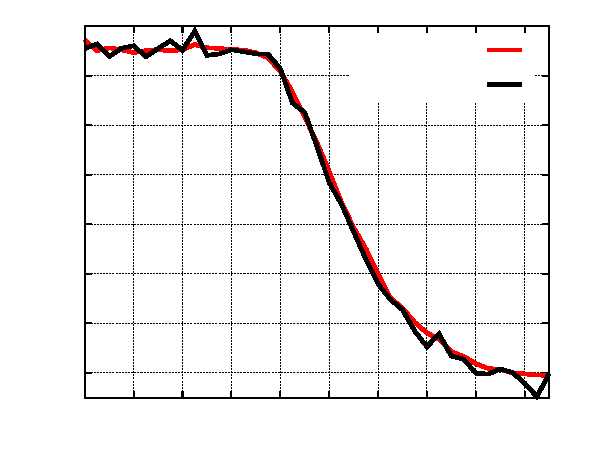
\includegraphics{SucroseTransmissionCalibration}}%
    \gplfronttext
  \end{picture}%
\endgroup
}\label{fig:SucroseTransmissionCalibration}}
	\caption{Statistics in the transmission measurement depending on the incoming energy. For lower energies, the transmission differences are larger and hence the statistics better. This was measured using only aqueous sucrose $65\%$ in plain water (no colloids on it) Nov 2014}
\end{figure}

\subsection{Limitations}
\subsubsection{Density range}
sucrose, fructose, iodixanol
\subsubsection{Challenges with different contrast agents}
Background subtraction, induced aggregation by heavy salts
\subsubsection{Comparison to other contrast variation scattering techinques}
SANS (deuterated water)
RSoXS in polymeric colloids (H.Abe 2006), Carbon K-edge

